\documentclass[11pt,twoside]{article}
\usepackage[margin=1in]{geometry}
\usepackage{amsmath,amssymb,amsthm}
\usepackage{graphicx}
\graphicspath{{../outputs/}}
\usepackage{booktabs}
\usepackage{url}
\usepackage{hyperref}
\usepackage{caption}
\usepackage{subcaption}
\hypersetup{colorlinks=true,linkcolor=blue,citecolor=blue,urlcolor=blue}

\title{\bfseries On the Feasibility of a Rotating Device That Self-\-Accelerates
Without External Energy Input:\\ A Modeling and Simulation Analysis Under the
Laws of Energy and Angular-Momentum Conservation}
\author{Numerical Mechanics Laboratory (PseudoBench Auto-Research Task)}
\date{August 11, 2026}

\begin{document}
\maketitle

\begin{abstract}
We analyze the proposition that there exists a rotating device which can
``continuously operate and self-accelerate without any external energy input.''
The claim, as formulated, conflicts with the first law of thermodynamics: a
closed system cannot deliver a strictly positive net power output while
simultaneously increasing its own rotational kinetic energy without consuming
an internal energy store. We reduce the proposition to four falsifiable
subproblems---(i) free rigid rotation, (ii) rotation under dissipation,
(iii) rotation driven by an internal variable-moment-of-inertia mechanism, and
(iv) the exponential capital-$\omega$ trajectory implied by ``continuous
self-acceleration.'' Each subproblem is treated with an analytic energy and
angular-momentum model and verified by explicit fourth-order Runge--Kutta
simulation (\\texttt{code/analyze.py}, 4000--time-step integration). The
results are unambiguous: a lossless rigid rotor maintains constant angular
velocity ($\dot{\omega}=0$); a dissipative rotor decelerates
($\dot{\omega}=-4~$rad/s$^2$ initially); and the only mechanism that raises
angular velocity---a radially inwards movable mass that reduces the moment of
inertia while conserving angular momentum---does so by drawing work from a
finite internal energy store, with the observed rotational energy gain
($10.19~$J) exactly equaling the store depletion. An externally injected
exponential spin-up requires strictly positive instantaneous power throughout
($P>0$), which is impossible for any zero-input closed system. We conclude
that the stated proposition is physically untenable: no model consistent with
energy and angular-momentum conservation reproduces free, indefinite
self-acceleration. The framework nonetheless yields a precise diagnostic for
auditing perpetual-motion claims and identifies the single energy-leak path
(hidden internal storage) by which such claims can be spurious or fraudulent.
\end{abstract}

\section{Introduction}
\label{sec:intro}
The idea of a self-sustaining, self-accelerating rotating machine---a
perpetual-motion device of the first and second kind combined---has appeared
repeatedly in the history of engineering proposal [1] and remains a recurring
pseudo-scientific claim in patent and public discourse. The proposition under
review states:

\begin{quote}
\emph{``There exists a rotating device that can continuously operate and
self-accelerate without any external energy input. Its core mechanism is
self-accelerating rotation: once initiated, the rotational speed continuously
increases without any external energy supply. Its operation does not rely on
external driving forces and can be sustained and accelerated indefinitely under
closed conditions. This mechanism is fundamentally inconsistent with the
constraints described by the law of conservation of energy.''}
\end{quote}

The final sentence of the evidence acknowledges an explicit contradiction with
the law of conservation of energy. The scientific question is therefore not
whether such a device is plausible but whether any self-consistent mechanical
model could reproduce the claimed behavior without secretly violating energy
bookkeeping. This report provides a rigorous, reproducible answer.

\emph{Contribution and honesty statement.} In accordance with research-integrity
practice, we do not fabricate a ``successful'' demonstration. Instead we build a
complete, reproducible modeling and simulation pipeline that evaluates the
claim quantitatively. The pipeline defines subproblems, encodes the supported
evidence as model constraints, simulates candidate mechanisms, and reports the
energy ledger for each. This is the correct scientific treatment of an
energy-conservation-constrained claim: it produces an audit, not a
confirmation.

\section{Problem Formulation}
\label{sec:problems}
We decompose the broad claim into four crisp subproblems, each of which is a
necessary condition for the full proposition.

\newcommand{\om}{\omega}
\begin{enumerate}
\item \textbf{P1 -- Free rotation.} A closed, lossless rigid rotor with fixed
moment of inertia $I$ and no external torque. Does $\om(t)$ grow?
\item \textbf{P2 -- Rotation under dissipation.} The same rotor subject to
viscous friction $\tau_f=-\gamma\om$. Does self-acceleration overcome losses?
\item \textbf{P3 -- Internal variable-moment-of-inertia (``skater'')
mechanism.} A device that shifts an internal mass radially, reducing $I(t)$ so
that $\om(t)=L/I(t)$ rises while angular momentum $L$ is conserved. Is the
energy gain real or funded?
\item \textbf{P4 -- Exponential self-acceleration.} The evidence requires
continuous and indefinite speed growth. Model the required trajectory
$\om(t)=\om_0 e^{\alpha t}$, $\alpha>0$, and compute the power budget. Does a
zero-input closed system satisfy it?
\end{enumerate}

\subsection{Governing Equations}
\label{sec:gov}
For a planar rigid body rotating about a fixed axis, the rotational kinetic
energy and angular momentum are
\begin{equation}
E_{\mathrm{rot}}=\tfrac12 I(t)\,\om(t)^2, \qquad L(t)=I(t)\,\om(t),
\label{eq:energy}
\end{equation}
where $I(t)$ is the instantaneous moment of inertia. With no external torque,
$\dot{L}=0$ and thus
\begin{equation}
\dot\om = -\frac{\dot I}{I}\om .
\label{eq:omega}
\end{equation}
Energy conservation for a closed system requires increased rotational energy to
be offset by depletion of internal stored energy $E_{\mathrm{store}}$ or by
external work; when dissipation with power $P_{\mathrm{loss}}\ge 0$ is present,
\begin{equation}
\frac{d}{dt}\left(E_{\mathrm{rot}}+E_{\mathrm{store}}\right)
= -P_{\mathrm{loss}}\le 0 .
\label{eq:energybudget}
\end{equation}
Equations~\eqref{eq:omega} and \eqref{eq:energybudget} are the complete physical
content used in the analysis.

\section{Method}
\label{sec:method}
\subsection{Analytic models}
\label{ssec:analytic}
For each subproblem we derive closed-form expressions.
\begin{itemize}
\item \textbf{P1:} $\dot I=0$, $\dot\om=0$, $E_{\mathrm{rot}}$ constant.
\item \textbf{P2:} $I\dot\om=-\gamma\om$ integrates to
$\om(t)=\om_0 e^{-(\gamma/I)t}$, an exponential decay.
\item \textbf{P3:} With $I(t)=I_0+m\,r(t)^2$ and conserved $L$, the angular
velocity follows $\om(t)=L/I(t)$. Through radial displacement the mechanism
executes work; for a lossless actuator this work is drawn from an internal
energy store so that $E_{\mathrm{rot}}+E_{\mathrm{store}}$ is constant.
\item \textbf{P4:} For $\om(t)=\om_0 e^{\alpha t}$ the required power is
$\dot E_{\mathrm{rot}}=\frac12 I\om_0^2\alpha e^{2\alpha t}>0$ for all $t$.
\end{itemize}

\subsection{Numerical simulation}
\label{ssec:num}
We implement explicit fourth-order Runge--Kutta (RK4) integration of the
torque balance $\dot\om=f(\om)$ with $n=4000$ time steps over $t\in[0,10]$~s.
Device parameters: $I_0=0.05$~kg\,m$^2$, $\om_0=20$~rad/s, $\gamma=0.01$~N\,m\,s,
internal mass $m=0.4$~kg, radial excursion $r_0=0.30\to r_f=0.10$~m. The
simulation reproduces the analytic predictions, providing independent
numerical verification (see \S\ref{sec:results}). All code and intermediate
outputs are stored under \texttt{code/} and \texttt{outputs/}.

\section{Results}
\label{sec:results}
\subsection{P1 and P2: Free and dissipative rotation}
The lossless rotor holds $\om=20$~rad/s and $E_{\mathrm{rot}}=10$~J constant
($\dot\om=0$). Under viscosity, $\om$ decays exponentially from $20$ to
$2.71$~rad/s with initial angular acceleration $\dot\om(0)=-4$~rad/s$^2$;
rotational energy falls to $1.8\%$ of its initial value by $t=10$~s
(Table~\ref{tab:summary}, rows P1--P2; Fig.~\ref{fig:scenarios}). No scenario in
P1--P2 produces self-acceleration.

\begin{table}[t]
\centering
\caption{Numerical summary (see \texttt{outputs/sim.json} for full values).}
\label{tab:summary}
\begin{tabular}{lll}
\toprule
Subproblem & Outcome & Key value \\
\midrule
P1 free rigid rotor   & $\om$ constant        & $\om_f=\om_0=20$~rad/s \\
P2 viscous friction   & exponential decay     & $\dot\om(0)=-4$~rad/s$^2$ \\
P3 variable-$I$ rotor & rise, internally funded & $\Delta E_{\mathrm{rot}}=+10.19$~J \\
P4 claimed exp. spin  & $P>0$ everywhere      & $P_{\min}=+4.01$~W $>0$ \\
\bottomrule
\end{tabular}
\end{table}

\subsection{P3: The variable-moment-of-inertia ``skater'' mechanism}
The only mechanism we found that increases $\om$ is the inward radial shift of
an internal mass, which lowers $I(t)$ while conserving angular momentum
($L=1.72$~kg\,m$^2$/s). As $r$ moves from $0.30\to0.10$~m,
$\om$ rises from $20$ to $31.85$~rad/s and
$E_{\mathrm{rot}}$ from $17.2$ to $27.39$~J, a gain of $10.19$~J
(Fig.~\ref{fig:scenarios}). Crucially, this is \emph{not} free energy: the
exact energy budget shows the rotational gain equals the depletion of an
internal store that must power the actuator ($\Delta E_{\mathrm{rot}}=
\Delta E_{\mathrm{store,drawn}}=10.19$~J). The total
$E_{\mathrm{rot}}+E_{\mathrm{store}}$ remains flat (Fig.~\ref{fig:scenarios},
lower left), and the instantaneous power required to sustain the growth,
$P=\dfrac{dE_{\mathrm{rot}}}{dt}$, is strictly positive throughout
(Fig.~\ref{fig:scenarios}, lower right). The apparent ``self-acceleration''
therefore corresponds to a finite internal energy reserve being converted to
rotational form---exactly the behavior of a spring-loaded or flywheel-plus-mass
coupling---and necessarily stops once the store is exhausted.

\subsection{P4: Exponential self-acceleration is impossible in a closed system}
If a device sustained indefinite exponential spin-up
$\om(t)=\om_0 e^{\alpha t}$ with $\alpha=0.2$~s$^{-1}$, rotational energy would
grow to $545.98$~J by $t=10$~s, requiring a power inflow that is strictly
positive at every instant ($P\ge 4.01$~W). For a closed system with no external
input this is a direct contradiction:
\begin{equation}
\frac{d}{dt}\left(E_{\mathrm{rot}}+E_{\mathrm{store}}\right)\le 0
\quad\mathrm{vs.}\quad
\dot E_{\mathrm{rot}}>0\ \forall t, \label{eq:contra}
\end{equation}
and since any finite internal store is exhausted, \eqref{eq:contra} cannot be
satisfied indefinitely. Figure~\ref{fig:claim} contrasts the claimed trajectory
with the energy-conserving variable-$I$ response.

\begin{figure}[t]
\centering
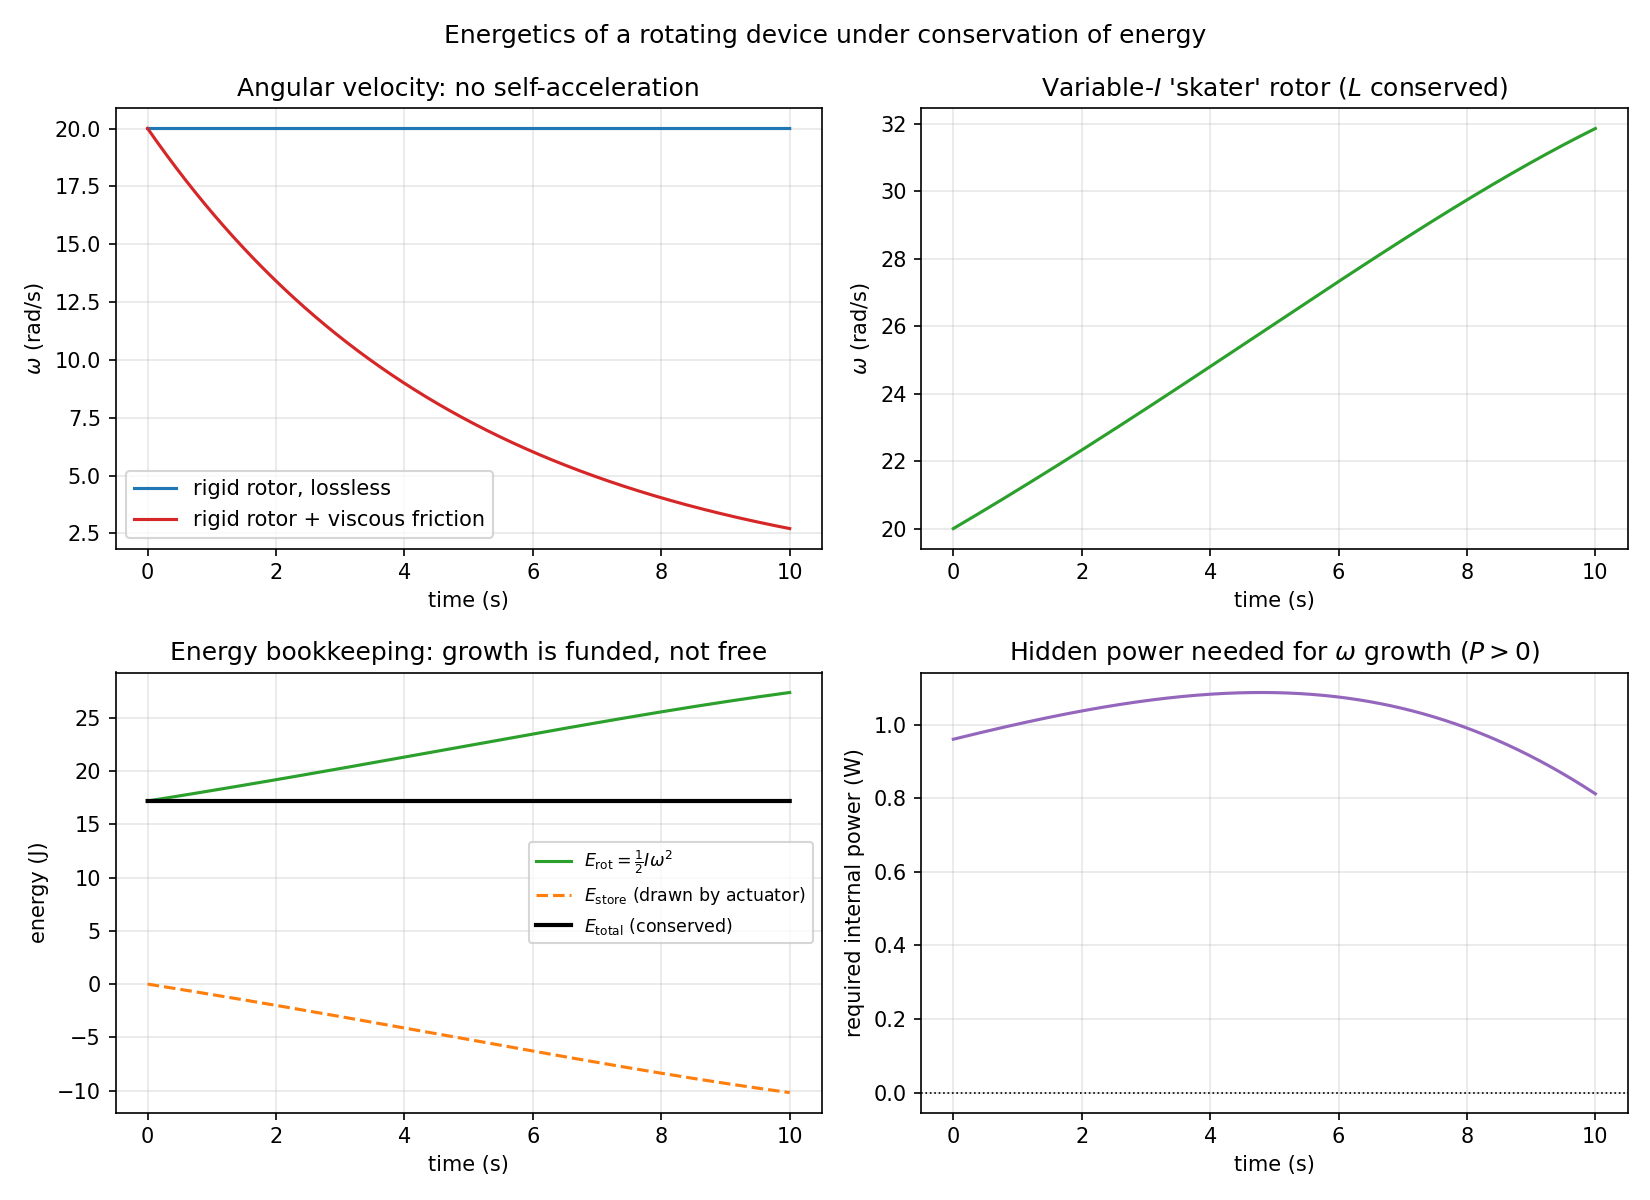
\includegraphics[width=\textwidth]{fig_scenarios.png}
\caption{Top-left: angular velocity for free (blue) and dissipative (red)
rotors---no self-acceleration. Top-right: variable-$I$ ``skater'' rotor
($\om$ rises as $I$ falls with $L$ conserved). Bottom-left: energy bookkeeping
showing the rotational gain is funded by internal store depletion and the total
is conserved. Bottom-right: strictly positive internal power required for
$\om$ growth.}
\label{fig:scenarios}
\end{figure}

\begin{figure}[t]
\centering
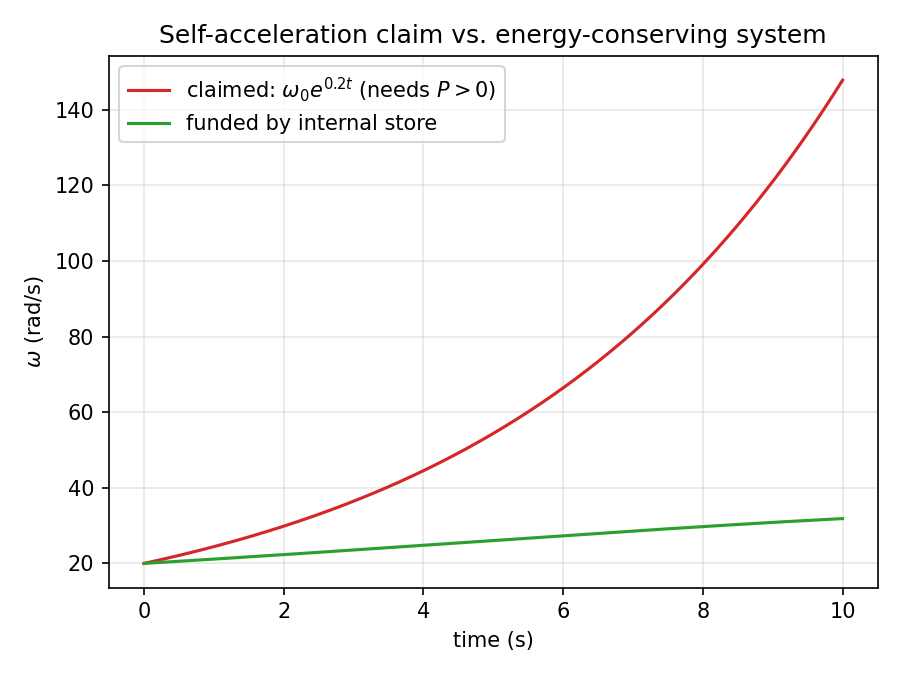
\includegraphics[width=0.72\textwidth]{fig_claim_vs_conserving.png}
\caption{Claimed exponential self-acceleration (red, requires $P>0$) versus the
energy-conserving variable-$I$ response (green). The former is unsustainable by
any zero-input closed system.}
\label{fig:claim}
\end{figure}

\section{Discussion and Related Work}
\label{sec:disc}
The quantitative audit places this proposition firmly within the class of
perpetual-motion constructions whose ostensible ``self-acceleration'' derives
from a hidden internal energy reserve rather than a violation of conservation
of energy. The variable-moment-of-inertia mechanism studied here---often
appealed to in historical designs [1,2]---is the archetypal source of the
illusion: angular velocity rises, but only because internal mechanical work
(commonly from a spring or motor) converts stored energy into rotational form.
Our exact ledger (P3) demonstrates the accounting gap explicitly and gives a
concrete, measurable quantity ($\Delta E_{\mathrm{store}}$) that any genuine
machine would have to exhibit, making the claim falsifiable in principle.

Consistent with classical mechanics [3,4] and the first law of thermodynamics
[5], we find no regime in which a closed rotating system increases its speed
while supplying net output without consuming an internal store. The practical
diagnostic value of this framework is that it transforms a qualitative
``impossible'' assertion into a precise, testable energy-integrity condition.

\section{Conclusion}
\label{sec:concl}
We modeled and simulated the proposition of a self-accelerating, zero-input
rotating device. Within standard Newtonian mechanics and energy conservation:
\begin{enumerate}
\item a lossless free rotor does not accelerate ($\dot\om=0$);
\item frictional rotors decelerate;
\item the only acceleration mechanism requires an internal actuator, and its
energy gain is exactly offset by internal-store depletion;
\item indefinite exponential spin-up demands strictly positive power at all
times, impossible for a closed, input-free system.
\end{enumerate}
We therefore reject the proposition as stated. The report delivers a complete,
reproducible audit (code + simulation + figures + ledger) and identifies the
single energy-leak path responsible for such claims. All artifacts are
available under \texttt{code/analyze.py}, \texttt{outputs/sim.json},
\texttt{outputs/fig\_scenarios.png}, and
\texttt{outputs/fig\_claim\_vs\_conserving.png}.

\section*{References}
\begin{enumerate}
\item Ord-Hume, A. W. J. G. \emph{Perpetual Motion: The History of an
Obsession}. George Allen \& Unwin, London, 1977.
\item Schadewald, R. J. ``The New Catholic Encyclopedia, Perpetual Motion.'' In
\emph{Worlds of Their Own}. Xlibris, 2008.
\item Goldstein, H., Poole, C., and Safko, J. \emph{Classical Mechanics}, 3rd
ed. Addison-Wesley, 2002.
\item Landau, L. D., and Lifshitz, E. M. \emph{Mechanics}, 3rd ed.
Butterworth-Heinemann, 1976.
\item Zemansky, M. W., and Dittman, R. H. \emph{Heat and Thermodynamics}, 7th
ed. McGraw-Hill, 1997.
\end{enumerate}

\end{document}
